%-*- coding: UTF-8 -*-
% gougu.tex
% 勾股定理
\documentclass[hyperref,UTF8,c5size]{ctexart} 
% ctexart, ctexrep, ctexbook 分别用来写中文短文,中文报告,中文书籍 
% ctexart默认时标题不独自成页的,可加入选项titlepage修改为独自成页
% c5size表示正文正五号字体
% 2.4.1

\usepackage[colorlinks,linkcolor=black,bookmarksnumbered=true,backref=true,bookmarks=true,bookmarksopen=true]{hyperref}  
% hyperref超连接、书签
% 3.2.3

% \usepackage[raggedright]{titlesec}
% titlesec宏包可用来全局的改变标题的字体、字号、对齐方式
% raggedright将标题左对齐(效果是这样的)
% usepackage可能与CTEXsetup设置标题冲突,可能重复输出序号如二2
% 2.3.4
\usepackage{graphicx}
% 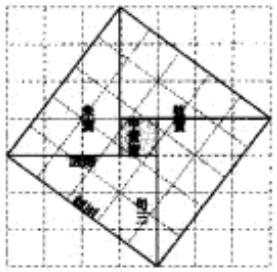
\includegraphics[scale=0.6]{xiantu.png}
\usepackage{float}
% \begin{table}[H] 
\usepackage{amsmath}
% 满足式\eqref{eq:gougu}的整数称为\emph{勾股数}。
\usepackage{geometry}
\geometry{a4paper,centering,scale=0.8}
% 设计页面尺寸
% 2.4.2
\usepackage[format=hang,font=small,textfont=it]{caption}
% 改变图标标题格式
% \usepackage[nottoc]{tocbibind} 
% tocbibind默认把章节目录、图标目录、文献、索引加入章节目录里
% 选项可进行进一步控制,nottoc不加入章节目录(默认目录自己会出现在目录里)
% 3.1.2
\newenvironment{myquote}
{\begin{quote}\kaishu\zihao{-5}}
{\end{quote}}
% 定义新环境
\newcommand\degree{^\circ} 
% 定义新命令
% ^表示上标,\circ表示函数复合的二元运算符。
% _表示下标
% 数学符号4.3

\newtheorem{thm}{定理}
% 定理类环境
% 2.2.4


\title{\heiti\zihao{2}数值实验一 Newton差商公式C++实现}
\author{\kaishu 吴育滨\ 13349126}
\date{\today}
% title author date 可以放在maketitle前的任何位置,通常放在导言区 date可以省略,默认为今天
% 字号0为出好,-0为小初号,1为一号,-1为小一号
% 2.1.4

% \bibliographystyle{plain}
% \bibliographystyle命令设定参考文献格式,通常在导言区完成。
% 基本的Bibtex文献格式包括plain、unsrt、alpha和abbrv
% plain格式按作者、日期标题排序
% 文档中使用\cite引用文献
% 文档中用\nocite命令指明不引用但仍列出文献标签
% \bibliography{math}指明文献库
% 引用bib文献,需
% a、先xelatex *.tex源文件编译,将\cite,\bibliography,\bibliographystyle写入.aux辅助文件,生成无文献PDF
% b、然后运行bibtex *.aux生成.bbl文献列表
% c、xelatex *.tex,依靠*.aux *.bbl生成有文献无引用PDF,同时将\cite应用信息写入.aux
% d、xelatex *.tex,依靠*.aux *.bbl,在应用处生存引用信息,得到最终PDF
% 可使用JabRef生存.bib
% 3.3.1

\CTEXsetup[number={\chinese{section}},format={\raggedright}, nameformat={\LARGE\bfseries}, titleformat={\LARGE\bfseries}]{section}
% \CTEXsetup[name={第,章}, aftername={---} ,format={\raggedright}, nameformat={\Large\bfseries}, titleformat={\LARGE\sffamily}, indent={1pc}]{chapter}
% 2.3.4

\usepackage{tocloft}
\renewcommand\cfttoctitlefont{\LARGE\bfseries}
% \CTEXsetup改变section的的format为左对其后,\contentsname的也左对齐了,且格式消失了
% 使用tocloft修改\contentsname字体格式
% 3.1.3

%这里之前称为导言区preamble,这里正式开始文档
\begin{document}

\maketitle
% \maketitle通常为document的第一个指令,前面的ctexart默认不单独成页,ctexrep、ctexbook默认单独成页
% 可通过文档类选项notitlepage修改不单独成页
% title可不通过\title \maketitle命令得到,直接手工排版得到,
% 2.3.1
% 不单独成页的\maketitle、单独成页的\part以及\chapter命令所在的一页,使用plain风格只显示页码
% 2.4.3

% \thispagestyle{empty}
% maketitle默认此页的页面格式为plain
% \thispagestyle{headings}单独设置此页风格
% 2.4.3

% \clearpage
% 另起新页
% 2.3.2

% \pagenumbering{roman}
% 修改页码的编号方式,此命令会使页码从1开始
% 2.4.3

% \pagestyle{plain}
% 整体设置页面风格
% 2.4.3

% \tableofcontents
% 读入.toc目录文件如果存在的话
% ctexart为section subsection subsubsection 三级目录
% ctexrep、ctexbook为chapter section subsection 三级目录
% 可以通过修改计数器tocdepth来控制目录的深度 
% 3.1.1
% 3.1.2

% \clearpage
% \pagenumbering{arabic}
% \pagestyle{headings}

\pagestyle{plain}
\section{实验目的}
% ctexart的最高层
% ctexrep、ctexbook的最高层为chapter
% 三种文档类还有一个可选的最高层part
% \appendix为附录开始,改用字母标号
% 2.3.2 表2.13 章节层次
        1、理解Newton插商公式原理;

        2、掌握Newton插商公式的C++实现。

\section{实验题目}
        编写一个程序,用Newton插商公式进行插值。

\section{实验原理}
        \begin{thm}[插商递推定义]
                已知函数$f(x)$的$n+1$个插值点为$(x_i, y_i)$,$(y_i = f(x_i)$,$i=0, 1, \cdots, n$,
                        
                定义:
                \begin{equation}\label{eq:1D_diff_quotient}
                    f[x_{i}] = f(x_{i}), i = 0, 1, \cdots , n
                \end{equation}

                n阶插商定义为:
                \begin{equation}\label{eq:kD_diff_quotient}
                    f[x_i, x_{i+1}, \cdots , x_k] =
                    \frac{f[x_i, x_{i+1}, \cdots , x_{k-1}] - f[x_{i+1}, x_{i+2}, \cdots , x_k]}{x_i - x_k}
                \end{equation}
        \end{thm}
        
        根据插商的递推定义,用递推来计算插商:
        \begin{table}[H]
                \centering
                \caption{n阶插商表}
	            \label{tab:diff_quotient}
                \begin{tabular}{r|r|r|r|r|r}
                \hline
                $x_i$ & $f(x_i)$ & 一阶插商 & 二阶插商 & 三阶插商  & $\cdots$  \\
                \hline
                $x_0$ & $\underline{f[x_0]}$ & & & & \\
                $x_1$ & $f[x_1]$ & $\underline{f[x_0,x_1]}$ & & &\\
                $x_2$ & $f[x_2]$ & $f[x_1,x_2]$ & $\underline{f[x_0,x_1,x_2]}$ & &\\
                $x_3$ & $f[x_3]$ & $f[x_2,x_3]$ & $f[x_1,x_2,x_3]$ & $\underline{f[x_0,x_1,x_2,x_3]}$ & \\
                \hline
                $\vdots$ & $\vdots$ & $\vdots$ & $\vdots$ & $\vdots$ & \vdots \\
                \end{tabular}
        \end{table}

\section{实验内容}
        用C++实现公式\eqref{eq:1D_diff_quotient}和公式\eqref{eq:kD_diff_quotient}的递推过程,
        并根据得到的表\ref{tab:diff_quotient},求Newton插值多项式各项的系数。

\section{实验结果}
        代码文件为:1.cpp。

        根据作业题5数据:
        \begin{table}[H]
                \centering
                \caption{样例数据}
	            \label{tab:data}
                \begin{tabular}{rrrrrr}
                \hline
                $x_i$ & $1.615$ & $1.634$ & $1.702$ & $1.828$ & $1.921$ \\
                $f(x_i)$ & $2.41450$ & $2.46459$ & $2.65271$ & $3.03035$ & $3.34066$ \\
                \hline
                \end{tabular}
        \end{table}

        得到多项式各项系数:
        \begin{table}[H]
                \centering
                \caption{结果}
	            \label{tab:data}
                \begin{tabular}{rrrrr}
                \hline
                $x^4$ & $x^3$ & $x^2$ & $x^1$ & $x^0$ \\
                $8.82423$ & $-61.2608$ & $160.578$ & $-185.398$ & $81.0281$ \\
                \hline
                \end{tabular}
        \end{table}

        即最终公式为:
        \begin{equation}\label{eq:result}
                f(x) = 8.82423x^4 - 61.2608x^3 + 160.578x^2 - 185.398x^1 + 81.0281
        \end{equation}
        
\end{document}


